\documentclass[10pt]{report}

\usepackage{geometry}
\geometry{
	a4paper,
	margin=1in,
	footskip=0.25in
}

\usepackage{enumerate} % for enumerate counter
\usepackage{subcaption} % for subfigures
\usepackage{amsthm} % for QED
\usepackage{mathtools} % for delimiter

\usepackage{listings} % for code
\lstset{ 
	language=R,
	basicstyle=\footnotesize\ttfamily,
	numbers=none,
	stepnumber=1,
	numbersep=8pt,
	showspaces=false,
	showstringspaces=false,
	showtabs=false,
	frame=single,
	tabsize=2,
	captionpos=t,
	breaklines=true,
	breakatwhitespace=false
} 

\usepackage{float} % for figure [H]
\usepackage{booktabs} % for tabular
\usepackage{caption} % for \caption*
\usepackage[export]{adjustbox} % for valign=t
\usepackage{array} % for column type m
\usepackage{verbatim}
\usepackage{graphicx}
%\graphicspath{ {imgs/} }

\usepackage{fancyhdr}
\pagestyle{fancy}
\fancyhead[L]{\hwAuther}
\fancyhead[C]{\courseNo}
\fancyhead[R]{\hwNo}

\usepackage{amssymb}
\usepackage{amsmath}

%Cover
\newcommand{\courseTitle}{Introduction to Mathematical Modeling}
\newcommand{\courseNo}{Math 380}
\newcommand{\hwAuther}{Zhihao Ai}

\newcommand{\hwNo}{HW \#1}
\newcommand{\hwDate}{Due on 01/23}

\title{
	\courseTitle\\
	\hwNo\\
	\hwDate
}
\author{\hwAuther}
\date{}
%

%Custom
%\everymath{\displaystyle}
\setlength\parindent{0pt}

%Custom commands
\newcommand{\ds}{\displaystyle}
\newcommand{\ts}{\textstyle}

\newcolumntype{N}{>$ c <$} 
\newcolumntype{M}[1]{>{\centering\arraybackslash $}m{#1}<{$}}

\newcommand{\abs}[1] {\left| #1 \right|}

\DeclarePairedDelimiter\autoparen{(}{)}
\newcommand{\pa}[1]{\autoparen*{#1}}

\newcommand{\var} {\text{var}}

\newcommand{\m}[1] {\mathbf{#1}}

\begin{document}

\maketitle

\section*{Section 1.1}
\begin{enumerate}
	\item[3.]
	By examining the following sequences, write a difference equation to represent the change during the $n$th interval as a function of the previous term in the sequence.
	
	\begin{enumerate}
		\item [b.]
		\{2, 4, 16, 256\}
		\begin{align*}
			a_{n+1} &= a_n^2, \quad n=0,1,2,3,\dots\\
			a_0 &= 2
		\end{align*}
		where $a_n$ is the $n$-th term of the sequence.
		
		\item [c.]
		\{1, 2, 5, 11, 23\}
		\begin{align*}
			a_{n+1} &= 2 a_n + 1, \quad n=1,2,3,\dots\\
			a_0 &= 1\\
			a_1 &= 2
		\end{align*}
		where $a_n$ is the $n$-th term of the sequence.
	\end{enumerate}

	\item [10.]
	Your grandparents have an annuity. The value of the annuity increases each month by an automatic deposit of 1\% interest on the previous month's balance. Your grandparents withdraw \$1000 at the beginning of each month for living expenses. Currently, they have \$50,000 in the annuity. Model the annuity with a dynamical system. Will the annuity run out of money? When? \textit{Hint}: What value will $a_n$ have when the annuity is depleted?
	
	Denote the value of the annuity after $n$ months as $a_n$. Assuming the value of the annuity increases each month before the grandparents withdraw \$1000, we have
	\begin{align*}
		a_{n+1} &= a_n + 0.01 a_n - 1000, \quad n=0,1,2,3,\dots\\
		a_0 &= 50000
	\end{align*}
	where $a_n$ represents the value of the annuity after $n$ months. Since $a_{70}$ is the first negative term, the annuity will run out of money after 70 months.
	
	\item [12.]
	Your current credit card balance is \$12,000 with a current rate of 19.9\% per year. Interest is charged monthly. Determine what monthly payment $p$ will pay off the card in 
	
	\begin{enumerate}
		\item [12a.]
		Two years, assuming no new charges.
		
		Denote the credit card balance after $n$ months as $a_n$. A rate of 19.9\% per year is equal to 1.658\% per month. Assuming the interest is charged before the monthly payment is made, we have
		\begin{align*}
			a_{n+1} &= a_n +  0.01658 a_n - p, \quad n=0,1,2,3,\dots\\
			a_0 &= 12000
		\end{align*}
		To make $a_{24}$ less than or equal to 0, meaning the amount left to be paid is 0, $p$ is computed to be approximately \$610.16.
		
		\item [13a.]
		Two years, assuming each month you charge \$105.
		
		Assume \$105 is charged before monthly interset. We have
		\begin{align*}
			a_{n+1} &= 1.01658 (a_n + 105) - p, \quad n=0,1,2,3,\dots\\
			a_0 &= 12000
		\end{align*}
		The monthly payment $p$ is computed to be approximately \$716.91.
	\end{enumerate}
\end{enumerate}

\section*{Section 1.2}
\begin{enumerate}
	\item [2.]
	The following data represent the U.S. population from 1790 to 2010. Find a dynamical system model that fits the data fairly well. Test your model by plotting the predictions of the model against the data.
	
	Let $p_n$ denote the U.S. population $10 n$ years after 1790. Plot $p_n$ against $n$, $\Delta p_n$ against $p_n$, and $\Delta p_n$ against $(4\times 10^8  - p_n) p_n$ assuming the carrying capacity is 400 millions:
	\begin{figure}[H]
		\centering
		\begin{subfigure}[b]{.3\linewidth}
			\caption{$p_n$ vs $n$}
			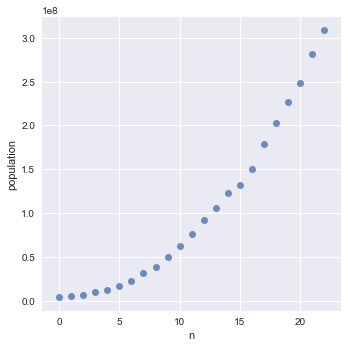
\includegraphics[width=\linewidth]{s1_2/p-n.png}
		\end{subfigure}
		\begin{subfigure}[b]{.3\linewidth}
			\caption{$\Delta p_n$ vs $p_n$}
			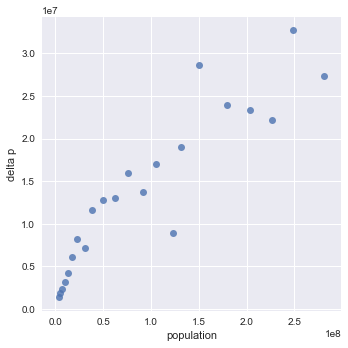
\includegraphics[width=\linewidth]{s1_2/dp-p.png}
		\end{subfigure}
		\begin{subfigure}[b]{.3\linewidth}
			\caption{$\Delta p_n$ vs $(4\times 10^8  - p_n) p_n$}
			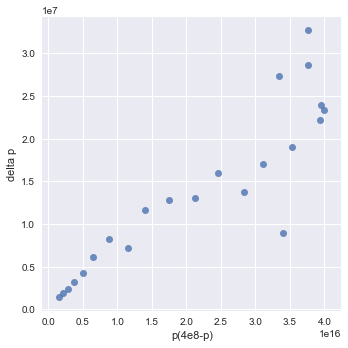
\includegraphics[width=\linewidth]{s1_2/dp-(c-p)p.png}
		\end{subfigure}
	\end{figure}
	Plot (a) shows that the population is not linear correlated with the year, so we turn to the first differences. There is roughly a linear relationship in (b) but it unreasonably predicts a non-stop increase of population. Taking into account the carrying capacity, we have figure (c) where the least square estimate of the slope of the regression line is $5.9145\times 10^{-10}$. Thus, we propose the model to be
	\begin{align*}
		p_{n+1} &= p_n + 5.9145\times 10^{-10} (4\times 10^8 - p_n) p_n, \quad n=0,1,2,3,\dots\\
		p_0 &= 3929000
	\end{align*}
	The predictions of the model against the data is shown below:
	\begin{figure}[H]
		\centering
		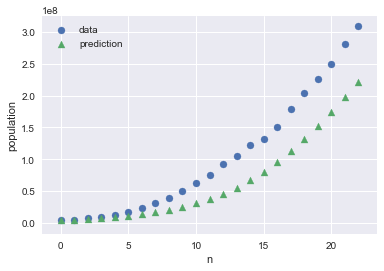
\includegraphics[width=0.5\linewidth]{s1_2/data-pred.png}
	\end{figure}
	
	\item [3.]
	Sociologists recognize a phenomenon called \textit{social diffusion}, which is the spreading of a piece of information, a technological innovation, or a cultural fad among a population. The members of the population can be divided into two classes: those who have the information and those who do not. In a fixed population whose size is known, it is reasonable to assume that the rate of diffusion is proportional to the number who have the information times the number yet to receive it. If $a_n$ denotes the number of people who have the information in a population of $N$ people after $n$ days, formulate a dynamical system to approximate the change in the number of people in the population who have the information.
	
	According to the assumption on the rate of diffusion, 
	\[
	\Delta a_n = k (N - a_n) a_n
	\]
	where $k$ is the estimated proportionality constant. Thus, we have the dynamical system
	\begin{align*}
		a_{n+1} &= a_n + k (N - a_n) a_n, \quad n=0,1,2,3,\dots\\
		a_0 &= c
	\end{align*}
	where $c$ is the initial number of people who have the information.
	
	\item [9.]
	The data in the table show the speed $n$ (in increments of 5 mph) of an automobile and the associated distance $a_n$ in feet required to stop it once the brakes are applied. For instance $n=6$ (representing $6\times 5 = 30$ mph) requires a stopping distance of $a_6 = 47$ ft.
	\begin{enumerate}
		\item 
		Calculate and plot the change $\delta a_n$ versus $n$. Does the graph reasonably approximate a linear relationship?
		\begin{figure}[H]
			\centering
			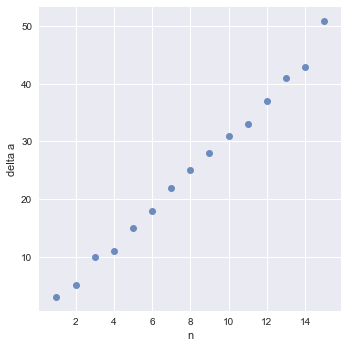
\includegraphics[width=0.4\linewidth]{s1_2/da-n.png}
		\end{figure}
		It reasonably approximates a linear relationship.
		
		\item 
		Based on your conclusions in part (a), find a difference equation model for the stopping distance data. Test your model by plotting the errors in the predicted values against $n$. Discuss the appropriateness of the model.
		
		Since $\Delta a$ is proportional to $n$, and the least square estimate of the proportionality constant is approximately 3.1395, we have $\Delta a = 3.1395 n$ and the following model
		\begin{align*}
			a_{n+1} &= a_n + 3.1395 n, \quad n=1,2,3,\dots\\
			a_1 &= 3
		\end{align*}
		The plots of predicted values and the errors are shown below:
		\begin{figure}[H]
			\centering
			\begin{subfigure}[b]{.4\linewidth}
				\caption{True and Predicted}
				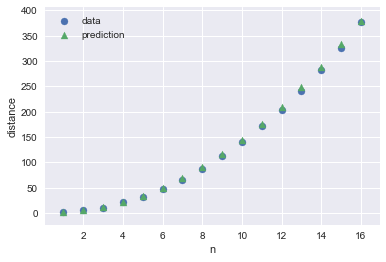
\includegraphics[width=\linewidth]{s1_2/9-data-pred.png}
			\end{subfigure}
			\begin{subfigure}[b]{.4\linewidth}
				\caption{Error}
				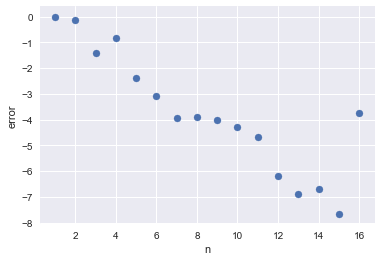
\includegraphics[width=\linewidth]{s1_2/9-error.png}
			\end{subfigure}
		\end{figure}
		The errors are small so the model is appropriate.
	\end{enumerate}
\end{enumerate}

\end{document}

